
%==== Document Setup (usthesis)======================================
\documentclass[report,                       %... Document type
				12pt,oneside,openany,a4paper, %... Layout
				a5block,                      %... A5 type block
				afrikaans,english            %... English default language
				]{usthesis}
				
%
% PLEASE read the USthesis documentation for the class options
% and how to set line and paragraph spacing
%

%==== Language setup ================================================
\usepackage[latin1]{inputenc}%................... Recognizes �, �, etc
\usepackage{babel}%.............................. Language setup

%==== Math setup ====================================================
\usepackage{amsmath}%............................ Advanced math (before fonts)
\usepackage{algorithm}
\usepackage[noend]{algpseudocode}
%\usepackage{amssymb}%............................ AMS Symbol fonts
\usepackage{siunitx}%............................	SI units

%==== Font setup (default is Computer Modern) =======================
\usepackage[T1]{fontenc}%........................ Type 1 fonts
\usepackage{textcomp}%........................... Additional text character
\usepackage{bm}%................................. Bold math symbols (after fonts)

%==== Ref's, Bib's and Nomencl ======================================
\usepackage{usnomencl}%.......................... List of symbols (in usthesis pack)
\usepackage{usbib}%.............................. Bibliography    (in usthesis pack)
\bibliographystyle{usmeg-a} 
\renewcommand\bibfont{\small}

%% For usmeg-a, the bib is a list of references. If you
%% are using usmeg-n comment out the following lines
\addto{\captionsafrikaans}{\renewcommand{\bibname}{Lys van Verwysings}}
\addto{\captionsenglish}{\renewcommand{\bibname}{List of References}}

%==== Graphics and Color ============================================
\usepackage{graphicx}%........................... Graphicx loaded in usthesis
\usepackage{color}%.............................. Color setup
\usepackage{caption}
\usepackage{subcaption}


%==== Table editing ============================================
\usepackage{multirow}
\usepackage{tabularx}

%==== Additional USthesis packages ==================================

\usepackage{ussummary}%.......................... Mech Eng summary page (in usthesis pack)

%==== Local Defs ====================================================
\makeatletter

%
% Please insert user defined commands here
\def\BState{\State\hskip-\ALG@thistlm}
% and NOT in the document itself!
%

\makeatother
%==== Title Page ====================================================

\title{Navigation and Control of an Unmanned Surface Vessel}


\author{}{L.E.V. \ Kingwill\\20725728}
\subject{Mechatronic Project 488}


\ReportDescript{Final Report}

\address{Department Mechanical and Mechatronic Engineering,\\
	Stellenbosch University,\\
	Private Box X1, Matieland 7602.}

\studyleader{Prof Jaco \ Versfeld}

\setdate{07}{2022}

%====================================================================%
%                 T H E   M A I N   D O C U M E N T                  %
%====================================================================%
\begin{document}

\frontmatter%========================================================

\TitlePage
%\CopyrightPage
\begin{Summary}{Plagiarism Declaration}
	I have read and understand the Stellenbosch University Policy on Plagiarism and the definitions of plagiarism and self-plagiarism contained in the Policy [Plagiarism: The use of the ideas or material of others without acknowledgement, or the re-use of one's own previously evaluated or published material without acknowledgement or indication thereof (self-plagiarism or text-recycling)].\par
	\vspace{0.4cm}
	I also understand that direct translations are plagiarism, unless accompanied by an appropriate acknowledgement of the source. I also know that verbatim copy that has not been explicitly indicated as such, is plagiarism.\par
	\vspace{0.4cm}
	I know that plagiarism is a punishable offence and may be referred to the University's Central Disciplinary Committee (CDC) who has the authority to expel me for such an offence.\par
	\vspace{0.4cm}
	I know that plagiarism is harmful for the academic environment and that it has a negative impact on any profession.\par
	\vspace{0.4cm}
	Accordingly all quotations and contributions from any source whatsoever (including the internet) have been cited fully (acknowledged); further, all verbatim copies have been expressly indicated as such (e.g. through quotation marks) and the sources are cited fully.\par
	\vspace{0.4cm}
	I declare that, except where a source has been cited, the work contained in this assignment is my own work and that I have not previously (in its entirety or in part) submitted it for grading in this module/assignment or another module/assignment.\par
	\vspace{0.4cm}
	I declare that have not allowed, and will not allow, anyone to use my work (in paper, graphics, electronic, verbal or any other format) with the intention of passing it off as his/her own work. \par
	\vspace{0.4cm}
	I know that a mark of zero may be awarded to assignments with plagiarism and also that no opportunity be given to submit an improved assignment.\par
	\vspace{2cm} 
	
	
	\noindent%
	\parbox{.5\textwidth}{%
		Signature:\quad\dotfill\par
		\hfill L.E.V.\ Kingwill \hspace{1.2cm}\null\par
		\hfill 20725728 \hspace{1.2cm}\null}
	
	
	\vspace{1cm}
	\noindent%
	\parbox{.5\textwidth}{%
		Date:\quad\dotfill\par}
\end{Summary}
%*** Summary Heading ************************************************
\begin{Summary}{Executive Summary}
	
	\noindent
	\begin{tabular}{@{}ll@{}}
		\textsf{Student:}    &  L.E.V\ Kingwill \\
	\end{tabular}
	
	%*** The Summary table **********************************************
	\begin{SumTable}
		\hline %=============================================================
		\hline
		\SumHead{Title of Project}\\
		\hline%=============================================================
		Navigation and Control of an Unmanned Surface Vessel.\\
		
		\hline%=============================================================
		\SumHead{Objectives}\\
		\hline%=============================================================
		The development of an independent navigation and control system that can be implemented on an unmanned surface vessel that uses electrical thrusters for propulsion and steering.\\
		
		\hline%=============================================================
		\SumHead{What is new in this project?}\\
		\hline%=============================================================
		A new control system is going to be created to control the power to the thrusters and thereby steer the vessel. Building on this a navigation system will be created so that the vessel can navigate to a designated point autonomously.\\
		
		\hline%=============================================================
		\SumHead{If the project is successful, how will it make a difference?}\\
		\hline%=============================================================
		With a successful navigation and control system, the system could be moved to vessels with better range and seafaring ability and these unmanned vessels can be used for research data collection, patrolling and search and rescue.\\
		
		\hline%=============================================================
		\SumHead{What contributions have/will other students made/make?}\\
		\hline%=============================================================
		N.A.\\
		
		\hline%=============================================================
		\SumHead{Which aspects of the project will carry on after completion and why}\\
		\hline%=============================================================
		For the vessel to be completely autonomous, a further project should investigate an obstacle avoidance system and power regeneration. This will be beneficial to avoid other sea vessels as well as fixed obstacles such as rocks and the shore. The power regeneration will extend the range of the vessel.\\
		
		\hline%=============================================================
		\SumHead{What arrangements have been/will be made to expedite contiuation?}\\
		\hline%=============================================================
		All the research and project documents will be archived with the university and the code-base will be thoroughly commented for ease of understanding.\\
		
		\hline%=============================================================
	\end{SumTable}
	
	%*** Signatures *****************************************************
	
	\vspace{1.5cm}
	\SumSignatures
	
\end{Summary}

\endinput

%\chapter{Abstract}
The aim of this project is to design and build a prototype control system for an unmanned surface vessel (USV). The system would make use of sensory equipment such as GPS and an electronic compass to aid in the navigation of the vessel. The vessel is designed to have an manual control mode to test the PWM signal used to power the thrusters, the power output of the thrusters and steering of the vessel. The autonomous control mode would navigate to given GPS coordinate points using the data from the external sensors. \par
Much of the hardware is outside of the scope of the project and was sourced or made by the Stellenbosch Electrical Engineering workshop. The hardware is explained to add context of how the system as a whole operates.\par
An Arduino microcontroller is used as the microcontroller due to its extensive libraries and user-friendly software environment. The data is retrieved from the sensors using mostly Arduino libraries and the control logic behind the novel control software is explained with the help of pseudo code and logic diagrams.\par
Each individual system is isolated and tested before the overall system is tested. All systems performed well in their individual tests however, the thrusters were slightly underpowered for the weight of the vessel. When testing the final system the weather conditions were not ideal, however the system still performed well and navigated to all the prescribed points.

\tableofcontents
\listoffigures
\listoftables
%\include{nomenkl}

\mainmatter%=========================================================

\numberwithin{equation}{chapter}%(from amsmath)
\numberwithin{figure}{chapter}  %
\numberwithin{table}{chapter}   %

\chapter{Introduction}
\section{Background}
As technology has improved over the years, processes and systems have become more automated. Initially factories were replacing manual labour with automated machines but recently companies have been investigating self-driving cars and trucks. All over industries tasks are being automated or done remotely with fewer human involvement. \par
\vspace{0.6cm}
The ocean is the perfect area for unmanned surface vessels (USV) to be used as many of the issues faced with autonomous land vehicles such as self-driving cars are mitigated by open water. On the open water one gets a 360° of the surroundings of the vehicle and although there can still be high volumes of traffic in certain areas such as commercial shipping lanes, due to the expanse of the ocean these high traffic areas are avoidable. Finally, and probably the most desirable mitigating factor is that where a surface vehicle would need to look where the road surface is to follow it, an ocean vessel can move directly from point to point on any piece of water. \par
\vspace{0.6cm}
In South Africa there is a growing need to USVs with regards to ocean research and conservation. There has been a growing use of acoustic sensory systems to track dolphins and whales around the world. By combining this with the technology of USVs, a far larger area can be surveyed. \par
\section{Objectives}
This project will focus on the navigation and propulsion control of the USV. This is the building block of the USV upon which a future project can build by adding an obstacle avoidance system or renewable power sources to keep the USV operational for longer. This project will have the following objectives:
\begin{enumerate}
	\item Design and manufacture an electric surface vessel.
	\item Designing and manufacturing the control system that will give a pilot manual control over the electric surface vessel.
	\item Building on the manual control and implementing navigation control so that the electric surface vessel.
\end{enumerate}
\section{Motivation}
Currently the marine community is using these acoustic systems as stationary systems. By using the USV in conjunction with the USV the area that is studied can be greatly increased with fewer acoustic platforms as have been used in passed projects. Furthermore, the technology can be adapted for use in other industries such sonar surveying, defence and search and rescue. The use of USVs is becoming more prominent as a USV can be cheaper to operate and therefore organisations can either save costs in the case of sonar and acoustic research or in the case or marine patrols and search and rescue, USVs can be used to fill up the ranks of vessels and close the possible.\par
\vspace{0.6cm}
The tasks previously mentioned are often time consuming and the crew of the assigned vessel need time to rest whereas a fully autonomous USV can operate constantly, stopping only to replenish its energy source and with further developments such as solar charging, USVs could begin to operate indefinitely, having to only come in for services or if there is a problem with the system.\par
\vspace{0.6cm}
This report will first look at what is a USV and what equipment and knowledge is required to for a USV. A review of literature around these technologies to offer a background and explain the concepts. Following on, the designed system is described before going into more detail on each component both hardware and electronics and the software and algorithms used in the system. Finally the report will describe how each system is tested and the results will be discussed before a conclusion on the system can be made.

\chapter{Literature Review}
\section{USV}
A USV is an unmanned surface vessel, and most often refers to an autonomous unmanned surface vessel \cite{Patterson2022}. With advancements in technology leading to unmanned drones and development into autonomous cars, unmanned surface vessels is a natural progression. There is a wide range of uses for unmanned surface vessels from research and surveying to rescue and military. The obvious benefit of an unmanned surface vessel over conventional naval vessels is the lack of any personal on-board. This means that the vessel can go into more dangerous situations such as rough weather without the risk loss of life \cite{Oceanalpha}. Furthermore, the vessel can operate 24hrs a day as long as it has an energy source. Finally, an unmanned surface vessel with the right power regeneration equipment can operate for months or years without having to resupply provided there are no unforeseen issues. Other benefits to an unmanned vessels, is that because they are often electrically powered as it is more easily controlled by software and they make use of renewable energy sources in order to remain self sufficient for long periods of time, a USV can have a carbon footprint as low as \SI{10}{\percent} of its manned counter part \cite{Fugro}.\par
The primary concern when trying to navigate open water is that need to know where you are and in which direction you need to go. Historically sailors used a combination of the stars as well as tracking their progress based on speed and time. However, this allows for inaccuracies as it does not account for cross winds and it can be difficult to determine your speed in stormy seas. In modern day naval navigation, GPS systems are used that can accurately pinpoint the location of the vessel anywhere in the world. The next step is to know in which direction you need to travel. Both historically and in modern day navigation you can use a mechanical compass that uses the earth's magnetic fields to determine which way is north and from which you can then determine in which direction you need to travel. \par
Using these navigation techniques, a USV needs at minimum, a GPS receiver to know its position and a digital compass to know its direction. However, there are other technologies that can be added to improve the performance and self-sufficiency of the USV. These include cameras and radar for surface obstacle avoidance such as debris, rocky outcroppings or ships \cite{Oceanalpha}. Sonar can be used to detect and avoid shallow waters or other obstacles below the waters surface. And solar and wind generators can be used to recharge the vessels power supply so that it can remain at sea for longer periods. 
\section{GPS}
\subsection{History of GPS}
\begin{figure}
	\begin{center}
		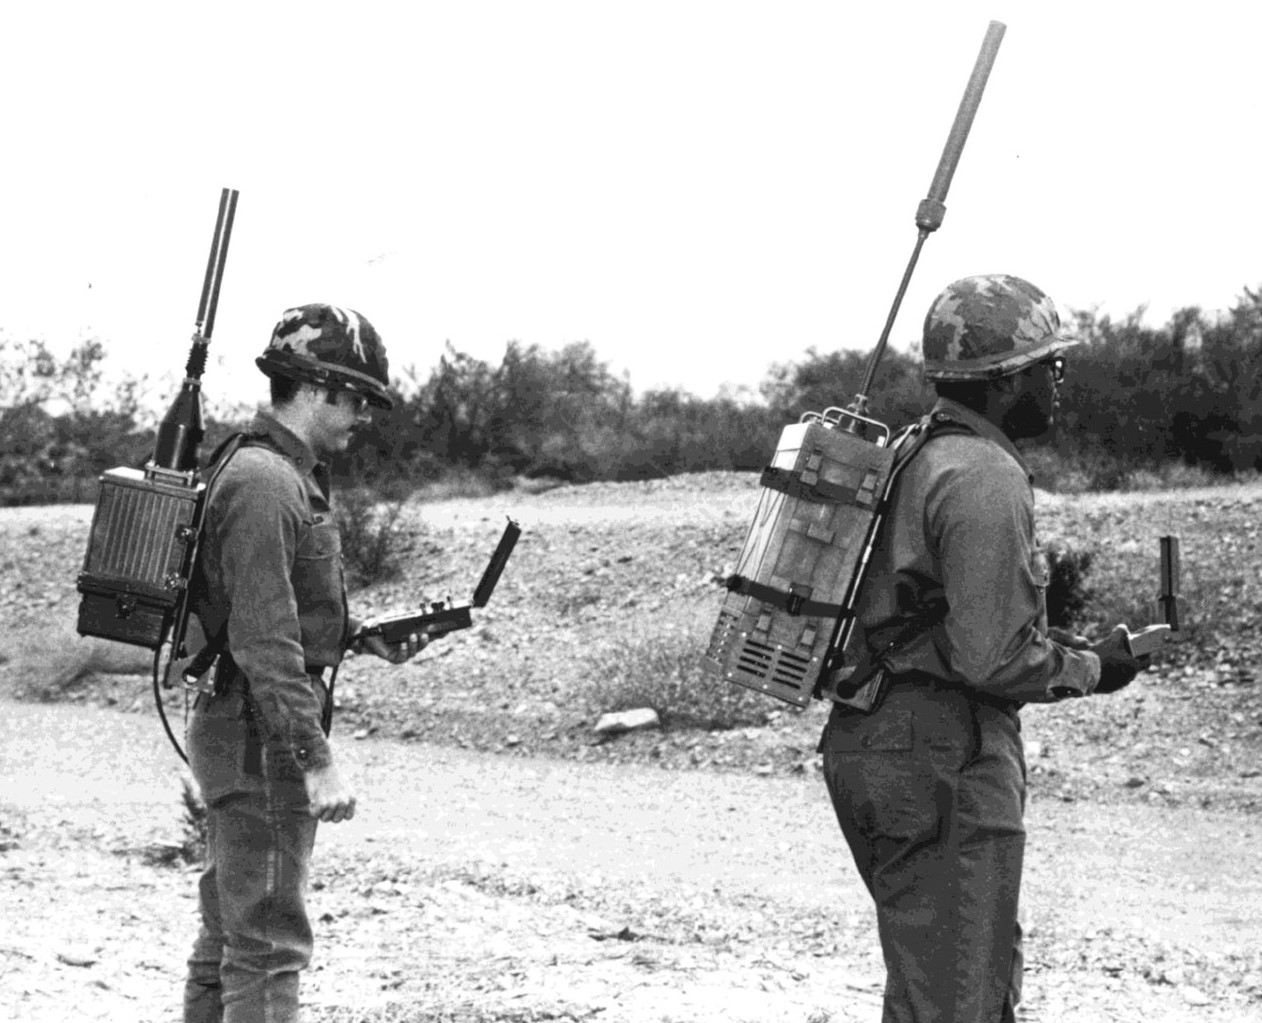
\includegraphics[width = 0.65\textwidth]{figures/historyGPS.jpg}
		\caption{Early GPS receivers were large, heavy devices. \cite{USAF1978}}
		\label{fig:2:histGPS}
	\end{center}
\end{figure}
Global Positioning System (GPS) is an everyday thing in our lives today and has become a luxury that most take for granted. There is GPS in our phones, laptops and even cars. We are using it to find directions on our commutes, hail taxis or ride shares and even for recreational sport, tracking how far we travelled.\par
\vspace{0.6cm}
The origins of GPS or rather any global satellite navigation system begins with the space race. It starts, in 1957, with the first satellite to successfully orbit the earth, the Russian satellite Sputnik. During its orbiting flight of the earth, Sputnik was emitting a radio signal which could be picked up on earth. During this orbit Scientists from John Hopkins University in America were monitoring the radio signals emitted by the Sputnik satellite when they saw the Doppler Effect in action with the radio signals, as the satellite drew closer, the radio signal frequency increased and vice versa. These scientists theorized that if they could determine the location of the satellite based on its signal frequency, the opposite would also be true, they could determine the location of a receiver on the ground given the satellites location. \cite{Aerospace2021}\par
\vspace{0.6cm}
The first instance of a global satellite navigation system was the Transit. It was developed in 1958 by the Advanced Research Projects Agency and the first satellite was launch in 1960. The Transit satellites were mostly used by the military, specifically the Navy's missile submarines. The program was transferred to the Navy during the mid-1960s. During this time there were further Transit satellites launched and by 1968 the entire constellation of Transit satellites was operational, a total of 36 satellites. \cite{Aerospace2021}\par
\vspace{0.6cm}
There was plenty of other research that was being conducted around the same time to improve on the current Transit. One such researcher was Phillip Diamond. Diamonds concept, from his study in 1963, lead to the Air Force forming a new satellite navigation program which he called 621-B. Further studies were undertaken by James Woodford and Hideyoshi Nakamura, which completed in 1966, proposed using four satellites. The use of four satellites would mean that the receivers no longer needed to be equipped with high-accuracy clocks. This was the first step in reducing the size and cost of the receivers. \cite{Aerospace2021} \par
\vspace{0.6cm}
There was a range of technological advancements that help progress the satellite navigation systems such as new bandwidth utilization techniques, advancements in computer and the introduction of solid-state microprocessors. These technological advancements helped reduce the size and weight of the GPS receivers to what we now know today, figure \ref{fig:2:histGPS} shows how large and cumbersome the early GPS receivers were. However, one significant technological advancement was the development of atomic clocks. This development led to another satellite navigation system known as Timation (Time Navigation). The third of three Timation satellites launched in 1974, became the first satellite equipped with an atomic clock, the previous two contained crystal oscillator clocks. The use of the atomic clock led to vast improvements in the accuracy of the navigation system and provided three-dimensional location coverage. \cite{Aerospace2021} \par
\vspace{0.6cm}
There were now three satellite navigation systems, and so when in the 1970s, the Department of Defence wanted a robust and stable system, the project team developed a new concept by cherry-picking the best aspects of all three, Transit, Timation and 621-B. This system was designated, Navigation System with Timing and Ranging (NAVSTAR), this was later changed to GPS I, the precursors to the GPS system we know today. The first NAVSTAR satellite was launched in 1978 and further satellites were launched in the following years, the system reaching its fully operational state with 24 satellites in 1993. \cite{Mai2017}\par
\vspace{0.6cm} 
Although the satellite navigation systems were operational and orbiting the earth, they were still used mostly by the military and the receivers were expensive. However, this began to change in 1983 when President Ronald Reagan authorized commercial airlines use of the NAVSTAR system. This was the start of civilian use of GPS. \cite{HistGPSProgram}
\par
\vspace{0.6cm} 
\subsection{Modern GPS}
The cost of GPS receivers began to decrease in the late-1990s, early-200s, the first cell phone containing GPS technology was released in 1999. The cost reduction can be attributed to the American government approving more non-military singnals as well as the technological advances in processors that was leading to cheaper processing chips. And naturally from the cheaper access, GPS use began to grow and putting more tax on the system which although upgraded to GPS II was not equipped to handle the modern requirments. In 2000 a plan was formed to add new signals to satellites that had not yet been launched in order to handle the increased use. Furhtermore, a new system was to be developed, GPS III, that could fully meet the modern requirements. The first of the GPS III satellites was launched in 2018 with a couple more in the following years and the remaining 6 to be launched by 2023. \cite{Aerospace2021}
\subsection{How GPS works}
\begin{figure}
	\begin{center}
		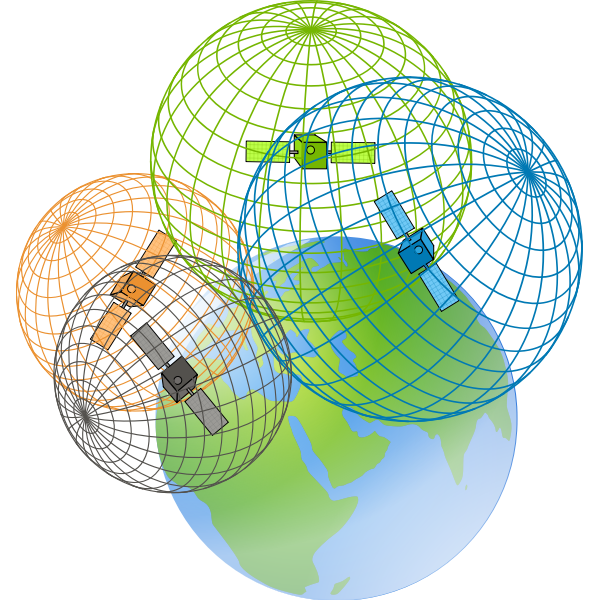
\includegraphics[width = 0.5\textwidth]{figures/GPStriangle.png}
		\caption{Distance spheres around each satellite intersect at one point}
		\label{fig:2:tiangleGPS}
	\end{center}
\end{figure}
There are a total of 31 GPS satellites currently sitting in a medium earth orbit. These are the satellites that are sending the radio signals that a GPS receiver can use to determine its location.\par
\vspace{0.6cm}
The signal that the satellites broadcast has a range of information that is used by receivers, this information contains data needed to determine the location of the satellite as well as the time that the signal broadcast, using the satellites atomic clock. Based on the time taken for the signal to reach the receiver and corrected for propagation delays or delays from the signal passing through the ionosphere and troposphere, the receiver can calculate the distance between itself and the satellite. This creates a sphere around the satellite upon which the receiver must lie. By adding in a second and third satellite and their distance spheres, there will be only two points of intersection between the three spheres. The one will be the receiver's location, while the other will be impossible location in space. However, to accurately calculate the distance, the receiver would have to have a synchronized atomic clock to determine exactly how long the signal takes to reach it. As it was mentioned earlier, highly accurate clocks were taken out of the receivers by adding a measurement from a fourth satellite to ensure that the distance calculation is accurate. Figure \ref{fig:2:tiangleGPS} illustrates the concept of the distance spheres and their intersection being the location of the GPS receiver. \cite{FederalAviationAdministration}
\section{Digital Compass}
Compasses have been used extensively over the past centuries for navigating, surveying, and map-making. The compass is thought to have been in use from around the 12th century in Europe and possibly earlier in east Asia \cite{Jones2019}. Although as many things have over the years been digitalized, so has the compass. The digital compass uses a technology called magneto-induction. This allows the digital compass to electronically detect the earth's magnetic field. Being as sensitive as it is an embedded microcontroller is needed to filter out any magnetic fields from ferro-magnetic materials or other electrical systems that are creating a magnetic field. \cite{AdvancedSafetyDevices2013}
\subsection{What is magnetic north}
\begin{figure}
	\begin{center}
		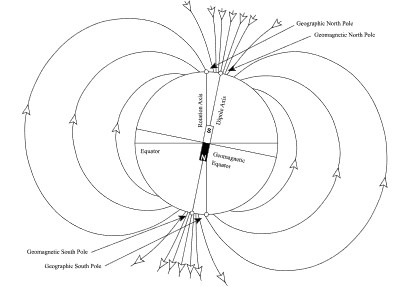
\includegraphics[width = 0.65\textwidth]{figures/tiltedDipole.jpg}
		\caption{The differentiation between magnetic and true north}
		\label{fig:2:magNorth}
	\end{center}
\end{figure}
True north is always fixed and is the direction that is directly in line with the north pole. However, compasses do not point to true north, they point to magnetic north. This is because a compass aligns itself with the magnetic field caused by the earth's magnetic core. The distinction between true north and the magnetic field at magnetic north is shown in figure \ref{fig:2:histGPS}. To further complicate the matter however, the earth's magnetic core experiences changes and these cause small shifts in the magnetic field around the earth. \cite{Jones2019}
\section{PWM}
\begin{figure}
	\begin{center}
		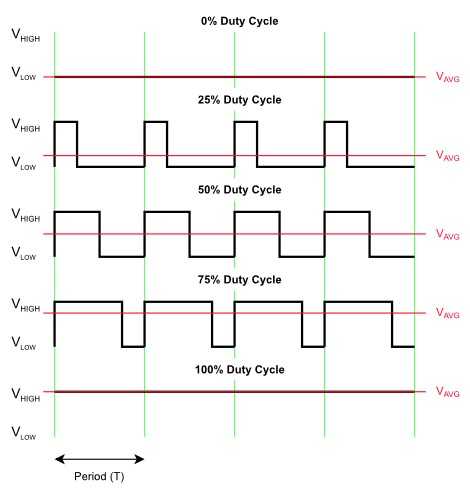
\includegraphics[width = 0.5\textwidth]{figures/PWM.jpg}
		\caption{Duty Cycle of PWM Signal}
		\label{fig:2:PWM}
	\end{center}
\end{figure}
Pulse Width Modulation (PWM) is a technique of using a digital signal to represent an analogue signal which is used to control analogue systems. The cost of switching a digital circuit between on (high) and off (low) is a cheaper alternative to creating an analogue circuit that will incur not drift over time. These PWM signals are mostly used in speed control of DC motors or controlling the brightness of lightbulbs. \cite{Christ2014}\par
\vspace{0.6cm}
PWM is a digital signal that is switched between high and low, leading to the generation of a square wave signal. The time that the signal goes high can be modulated to vary the power delivered to the system. Typically, microcontrollers are used to generate and control the PWM to power an external system. There are a few signal parameters that will be highlighted in this explanation of a PWM signal. The signal amplitude, this is the maximum voltage that can be supplied to the external system. If the microcontrollers output voltage is insufficient for the external system, the signal can be passed through an amplifying circuit to provide the required voltage. Secondly is the signal period, and therefore the frequency as they are inversely proportional, and is the total time for one signal wave to propagate. The frequency is set depending on the requirements of the system, but this frequency will be needed later to help with the calculation of the duty cycle. The duty cycle is the final parameter. The duty cycle is the ratio between the time the signal is high and the time the signal is low. It is always a value between 0 and 1, however, the duty cycle is often expressed as a percentage.\par
\vspace{0.6cm}
A PWM varies the voltage supplied to the system by varying the duty cycle. A small duty cycle means that the signal is high for a short portion of the signal period while a large duty cycle means that the signal is low for a large portion of the signal period. The system that is being supplied then uses the average voltage of this period. Therefore, a low duty cycle, a short high signal followed by a long low signal, would lead to a low average voltage. The variation in duty cycle and the associated average voltage is shown in figure \ref{fig:2:PWM}. \cite{Ibrahim2014}\par
\vspace{0.6cm}
To determine how long the signal must go high, the duty cycle is multiplied by the signal period. The duty cycle is often expressed as a percentage and so the duty cycle is the percentage of time that the signal is high. Therefore, by multiplying the duty cycle with the period gives the time for which the signal is pushed high (t1). Figure \ref{fig:2:PWMPulse} shows the relationship between t1, the time the signal is high, and T, the signal period.\par
\vspace{0.6cm}
\begin{figure}
	\begin{center}
		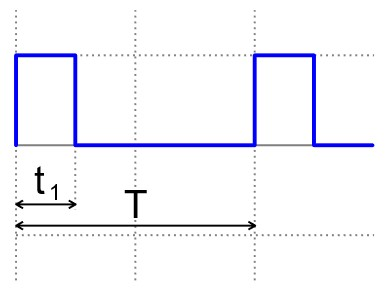
\includegraphics[width = 0.65\textwidth]{figures/PulseWideWave.jpg}
		\caption{The relation between the time the signal is high and the signal period.}
		\label{fig:2:PWMPulse}
	\end{center}
\end{figure}
\section{Analogue vs Digital Signals}
\begin{figure}
	\begin{center}
		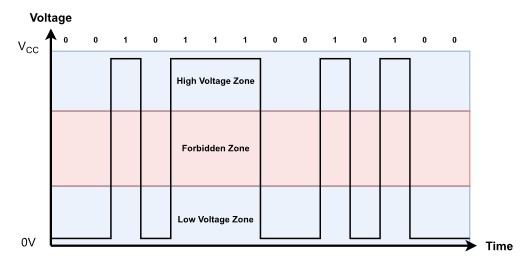
\includegraphics[width = 0.75\textwidth]{figures/DigitalSignal.jpg}
		\caption{A digital signal and its three zones.}
		\label{fig:2:digital}
	\end{center}
\end{figure}
Signals are used to convey data and information from point to point. For this project only electrical signals will be used although there are plenty of other mediums through which signals can be sent. There are two predominant signals that are used when regarding electrical signals, analogue and digital. \par
\vspace{0.6cm}
A digital signal, most simply represents discrete values, more precisely 2 discrete values. This makes digital signals perfect for conveying data in a binary data format but slightly more troublesome when more than two values are required. It will transmit a signal as either a low voltage, a zero, or a high voltage, a one. The low voltage is generally 0V while the high voltage is the voltage supply of the driving device. However, because voltages can have small fluctuations and will therefore not always be exactly 0V or equal to the nominal voltage, a range is pre-set whereby the receiving device can denote the value as low or high. A buffer zone is also incorporated, a voltage range around half the value of the nominal voltage, to prevent a small fluctuation in the voltage possibly altering the value of the signal. This buffer zone along with the area in which the signal can be read as high or low is shown in figure \ref{fig:2:digital}. This buffer is called the forbidden zone any signal received within the forbidden zone is considered floating and will be randomly assigned as either high or low.\par
\vspace{0.6cm}
An analogue signal on the other hand is continuous and where the digital signal ranged from 0 to an upper voltage, an analogue signal ranges from a low voltage to a high voltage. Typically, $±V_CC$, the voltage of the microcontroller, is used for these upper and lower limits. An example of a continuous analogue signal between $±V_CC$ is shown in figure \ref{fig:2:analogue}. An analogue signal can therefore transmit an infinite number of values between these limits. By assigning an upper and lower limit to the sensor that will transmit the data, a max min transformation can be computed, and the transformed value transmitted along the analogue signal. Because the analogue signal is continuous, it can also be used in tracking the change in a value over time by computing the integral of the signal wave.\par
\begin{figure}
	\begin{center}
		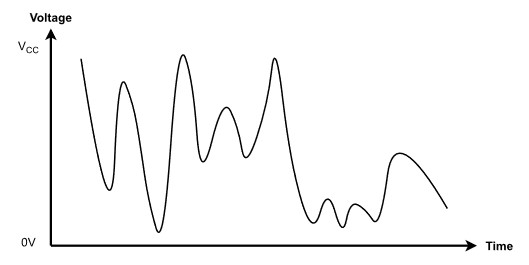
\includegraphics[width=0.75\textwidth]{figures/AnalogSignal.jpg}
		\caption{Analogue signal}
		\label{fig:2:analogue}
	\end{center}
\end{figure}



\chapter{Methodology and Design}
This chapter will describe the methodology used in the project. The project is mostly software based and so that will be the focus. However, there is a physical element in that of the vessel and the electrical hardware. The mechanical design and fabrication of the thruster mounts is outside the scope of this project and so it will be described only in terms of how it interfaces with the electrical hardware.\par
\section{Software Environment}
The microcontroller that was chosen for this project is a Arduino DUE. An Arduino microcontroller was chosen as there is a wide range of Arduino libraries available online, as well as several forums and code examples. Furthermore, the Arduino environment uses the C language. \par
\section{System Design}
	\subsection{Objective}
	The system needs to be designed to be deployed for long periods of time between servicing. The future addition of power regeneration such as solar or wind can be used to improve the deployable range and period of the vessel but the energy storage must be designed to handle an extended period of ‘dark time’, any time when the power regeneration is negligible. \par
	The vessel must be autonomous and having received a set of points before deployment, navigate between these points until retrieval. Even under non ideal circumstances the vessel should be able to correct its course and continue to navigate to the set points. \par
	This system is a proof of concept that is designed to be able sized up to a larger vessel. Therefore the prototype vessel should be able to handle any conditions that could be encountered in testing and all electronics should be sufficiently sealed so that no damage is incurred. It is not expected that the prototype vessel can handle rough and storm weather conditions.\par
	\subsection{Engineering Requirements}
	The prototype is a proof of concept that can be scaled up to a larger vessel and so a small vessel that can accommodate at least 2 people is required. This is preferred to a smaller vessel that cannot accommodate the weight of a person as the weight to power ratio of a small vessel would not be as representative and this could influence the steering capability of the vessel and therefore the control system.
	Furthermore, a working vessel is going to require a large battery bank and this is easily represented in a larger vessel. The energy source can then be scaled up by adding cells in both parallel and series to create the required power supply for the working vessel.\par
	The autonomous nature of the vessel means that the a electronic control system is required to control the vessel. Furthermore, there are several elements that are required to make up the system however, these are not integral to the autonomous nature of the system but integral to the system as a whole. All of these elements are listed in the table \ref{tab:3:elements} and will be further explained in the system description.\par
\section{System Description}
This section will give a broad overview of the system as a whole and describe the different sub-systems and their interactions. Several of these subsystems are outside the scope of the project but have been included to provide a foundation upon which the applicable detailed descriptions will build. \par
	\subsection{Hardware}\par
		\subsubsection{Vessel}
		The vessel is outside the scope of this project as it was acquired before the start of the project and the project was designed around the use of the vessel for testing. The vessel referred to in this project is a Spider 3, a small single hulled fibreglass boat. The vessel measures \SI{1.3}{\meter} $\times$ \SI{3.2}{\meter} and is rated to carry 4 people and a 15hp traditional outboard motor.\par
	\subsection{Electronics}\par
		\subsubsection{Arduino Due}\par
		\subsubsection{ESC}\par
		\subsubsection{PWM Signal}
		The thrusters are each controlled by a \SI{5}{\volt} PWM signal. There is limited information on the datasheet for the ESC and the signal boundaries, full forward, full reverse and neutral positions are described in the unconventional terms of the time that the signal is high. The values are shown in table \ref{tab:3:PWM}. Initially it was thought that the ESC operated at \SI{50}{\hertz}, however there was no response from the thruster at any duty cycle.\par
		\begin{table}[!ht]
			\begin{center}
				\caption{ESC boundaries and PWM duty cycle at various frequencies.}
				\label{tab:3:PWM}
				\begin{tabular}{|l|c|c|c|c|}
					\hline
					\multirow{2}{*}{Position} & \multirow{2}{*}{Time (\SI{}{\micro\second})} & \multicolumn{3}{c|}{Duty Cycle @}\\
					%\hline 
					& & \multicolumn{1}{c}{\SI{50}{\hertz}} & \multicolumn{1}{c}{\SI{60}{\hertz}} & \multicolumn{1}{c|}{\SI{500}{\hertz}}\\
					\hline
					Full Forward & 2000 & \SI{10}{\percent} & \SI{12}{\percent} & \SI{100}{\percent}  \\
					\hline
					Neutral & 1500 & \SI{7.5}{\percent} & \SI{9}{\percent} & \SI{75}{\percent}  \\
					\hline
					Full Reverse & 1000 & \SI{5}{\percent} & \SI{6}{\percent} & \SI{50}{\percent}  \\
					\hline
				\end{tabular}
			\end{center}
		\end{table}
		\vspace{0.4cm}
		In order to be sure that the correct PWM signal was being sent through and to be able to quickly vary both the frequency and the duty cycle, a PWM signal generator IC was connected to ESC and trial and error was conducted to determine that the ESC began responding to a signal above \SI{60}{\hertz}. It was then decided to push the frequency up to the maximum of \SI{500}{\hertz} as this would offers the finest control because it has the maximum allowable duty cycle difference between the signal boundaries.\par
		\vspace{0.4cm}
		The Arduino libraries contain a function that can output a PWM wave, given the duty cycle and the pin to output on as a parameter however, the default frequency of the Arduino DUE PWM pins is \SI{1000}{\hertz}. Therefore, the frequency had to be manually changed by changing the timer settings driving the PWM signal.\par
		\vspace{0.4cm}
		The information needed to change the timer settings is available in the Arduino Datasheet. The process to configure the PWM outputs is as follows. First, the peripheral clocks for timer channels 6 and 7 were enabled. Secondly, the pins input output controller on peripheral A needed to be disabled and the pins switch to peripheral type B. Then came the configuration of the timer itself. The channel mode was set to waveform mode using clock 1 with the counter being incremented on the rising edge. Furthermore, the waveform was set to UP mode (signal being set high) being triggered when the counter reached the register C (RC) value and the signal being cleared when the counter reached the register A (RA) value. Once the timer is configured, the RA and RC values can be filled and the interrupt set to trigger when the counter reaches RC. Finally, the channel control register is set to perform a software trigger, reset the counter and start the clock. There is also a interrupt handler that needs to be added where in the status register is read. This is done because the flags in the status register are automatically reset when the status register is read, at the end of every period.\par
		\vspace{0.4cm}
		The signal is being cleared when the counter reaches RA and set high when the counter reaches RC and so RC can be equated to the period of the signal and RA to the time when the signal is high. Using this and that the clock is set to clock 1 which is the MCU clock (MCK) divided by 2, the RA and RC can be expressed in terms of MCK, frequency and duty cycle as shown in equations \ref{eq:3:RC} and \ref{eq:3:RA}. RC is kept constant throughout while RA is changed to change the duty cycle of the PWM signal sent to the ESC and therefore control the ESC and thruster.
		\begin{equation}
			RC = \frac{\frac{MCK}{2}}{Frequency}
			\label{eq:3:RC}
		\end{equation}
		\begin{equation}
			RA = RC \times Duty Cycle
			\label{eq:3:RA}
		\end{equation}
		
		\subsubsection{Throttle and POT}
		The initial concept was to use two throttles that can move independently from each other and %item \ref{BOM:smallThrottle} in Appendix \ref{BOM} was
		two electronic throttles were 
		% remove comments when BOM is in place
		purchased to be used. However, when these components arrived, they were much smaller than they had appeared and they had very small range of movement. The next solution was to use two linear potentiometers (POT) and to build a throttle system that linked to the POTs. The workshop designed and built the throttle system.
		% as shown in figure \ref{fig:3:throttle}. 
		\par
		\vspace{0.4cm}
		The POT has three pins as shown in figure \ref{fig:3:POTdraw}, high voltage, ground and the output. The high voltage and ground are connected to the connections on either side and the output is connected to the middle. The output is therefore a voltage in the range of $V_{CC}$ to GND. The Arduino DUE pins are \SI{3}{\volt} tolerant and so the $V_{CC}$ is driven by \SI{3}{\volt} signal. \par
		\vspace{0.4cm}
		\begin{figure}[ht]
			\begin{center}
				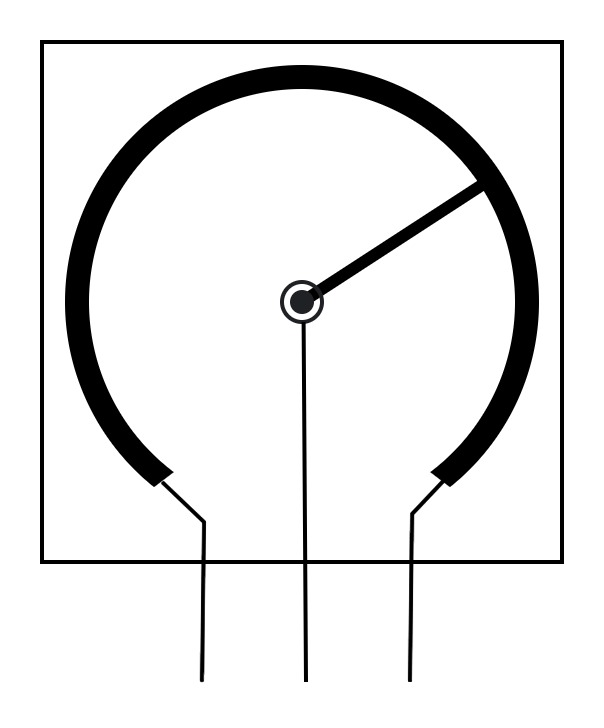
\includegraphics[width = 0.3\textwidth]{figures/POT.jpg}
				\caption{Fundamental illustration of a linear potentiometer}
				\label{fig:3:POTdraw}
			\end{center}
		\end{figure}
		The output of the POT is connected to analogue pins on the MCU and so the function, \textit{analogRead()} can be used to convert the analogue voltage into digital value using the built in ADC. The ADC has a 10 bit resolution and so the digital value is an integer in the range 0 to 1024 and the smallest discernible voltage change is \SI{3}{\milli\volt}. However, the design of the throttle does not use the full \SI{300}{\degree} range and so the physical limits needed to be measured to calibrate the throttles. The measured limits and centre points for the two throttles are shown in table \ref{tab:3:POT}. The neutral position is described by two values so that there is a neutral range that could easily be achieved by the users input. \par
		%\vspace{0.4cm}
		\begin{table}[ht]
			\begin{center}
				\caption{Measured physical limits and neutral range of the throttle POTs}
				\label{tab:3:POT}
				\begin{tabular}{|l|c|c|}
					\hline		
					\textbf{Throttle Position} & \textbf{Left POT} & \textbf{Right POT} \\
					\hline
					Full Forward & 677 & 700\\
					\hline
					\multirow{2}{*}{Neutral} &530 &540 \\
					&490 &500  \\
					\hline
					Full Reverse & 321 & 340 \\
					\hline
				\end{tabular}
			\end{center}
		\end{table}
		Using table \ref{tab:3:PWM} and \ref{tab:3:POT} a relationship can be created to determine the RA value for a given throttle position. Because the forward operation is in the duty cycle range \SI{75}{\percent} to \SI{100}{\percent}, the analogue input from the POT needs to be linearly mapped to represent an equivalent duty cycle in this range. Equation \ref{eq:3:dutyF} shows how this is done for the forwards operation. The same logic can be used to determine the duty cycle for reverse as equation \ref{eq:3:dutyR} shows. However, neutral is a set value that is written to RA whenever the throttle is within the neutral range.
		\begin{equation}
			Duty Cycle_{Forward} = 100 - (100-75)(\frac{POT_{MAX} - POT_{Input}}{POT_{MAX} - POT_{Neutral}})
			\label{eq:3:dutyF}
		\end{equation}
		\begin{equation}
			Duty Cycle_{Reverse} = 75 - (75-50)(\frac{POT_{Neutral} - POT_{Input}}{POT_{Neutral} - POT_{MIN}})
			\label{eq:3:dutyR}
		\end{equation}
		\subsubsection{GPS Module}
		%Item \ref{BOM:GPS} in appendix \ref{BOM} is the GPS module used. It
		The GPS module used is a PmodGPS and it
		%remove comments when the BOM is correctly added.
		has two connectors J1, which has 6 pins and J2 which has 2 pins. J1 is used to power the GPS module as well as connect to the MCU using UART communication with a baud rate of 9600, 8 data bits, no parity and 1 stop bit. The GPS module transmits a series of 5 sentences containing various information. Each sentence begins with a '\$GP' and then the specific message ID. The data is then sent through comma separated and finally ends with a checksum and the end of line characters <CR><LF>. For this project the 'RMC' sentence is the only sentence of interest as it contains all the necessary information, longitude, latitude, speed over ground in knots and course over ground in degrees. An example of the 'RMC' sentence is shown below.\par
		\vspace{0.2cm}
		\par
		\begin{center}
			\begin{tabular}{c}
				\small{\$GPRMC,064951.000,A,2307.1256,N,12016.4438,E,0.03,165.48,260406,3.05,W,A*55<CR><LF>}\\
			\end{tabular}
		\end{center}
		\vspace{0.4cm}
		The entire sentence is read by the MCU before it starts to pick out the specific data out of the string using the commas and full stops as the guide to what array position is what data. Each piece of data is then added to an instance of a GPS structure that can then be easily parsed to the navigation algorithm and easily analysed. The variables within the GPS structure are shown in table \ref{tab:3:GPSstruct}.
		\begin{table}[!hb]
			\begin{center}
				\caption{Variables and their types within the GPS structure.}
				\label{tab:3:GPSstruct}
				\begin{tabular}{|l|l|l|}
					\hline
					\textbf{Name} & \textbf{Type} & \textbf{Description} \\
					\hline
					UTC & int & Coordinated Universal Time in the format (hhmmss). \\
					\hline
					lat & int & The whole number portion of the latitude. \\
					\hline
					latDecimal & int & The decimal portion of the latitude. \\
					\hline
					n\_s & char & A character indicating North or South. \\
					\hline
					longi & int & The whole number portion of the longitude. \\
					\hline 
					longiDecimal & int & The decimal portion of the longitude. \\
					\hline 
					e\_w & char & A character indication East or West. \\
					\hline
					knots & float & The speed over ground in knots. \\
					\hline
					course & float & The course over ground in degrees. \\
					\hline
					date & int & The date in the format (ddmmyy). \\
					\hline
				\end{tabular}
			\end{center}
		\end{table}
	\subsection{Software}

\subsection{Thrusters and Energy Cells}
The propulsion system consists of two electric thrusters mounted at the back of the vessel. These thrusters are each capable of producing up to \SI{18}{\kilogram} of thrust. They are mounted onto the back of the vessel with a metal mount that is removable and height adjustable. Each thruster has a submersible ESC attached which is controlled by a \SI{5}{\volt} PWM signal. The ESC can drive the thruster in both forward and reverse direction.\par
\vspace{0.4cm}
The thrusters are powered by a battery bank of 4 Lithium Iron Phosphate cells. Each cell has a voltage of \SI{3.3}{\volt} and a capacity of \SI{100}{\ampere\hour}. The 4 cells are connected in series to provide \SI{12}{\volt}. The battery is connected to the thrusters through a smart battery management system (BMS) which has an allowable discharge current of \SI{100}{\ampere} and an allowable charge current of \SI{50}{\ampere}.
\subsection{Control System}
The control system is the intended scope of the project and consists of a manual and automated control. For manual control, there is a two lever throttle system that is used to control the thrusters. In automated control, the control system uses a GPS and digital compass to navigate to prescribed points. At the centre of this control system is the PCB motherboard containing the MCU, GPS and connections to both the throttle and the thrusters. 
\section{Control System}
The control logic of the control system is all implemented through the software on the Arduino MCU. This section will go into detail on logic and how that logic is carried out in software as well as the electronics that are used. 
%The source code that will be discussed can be seen in Appendix \ref{Code}

\chapter{Testing and Results}


\appendix%===========================================================

%
\chapter{Techno-Economic Analysis}
This appendix contains details on the cost of the project both in terms of materials and supplies as well as the cost of the Electrical Engineering workshop and the cost of a junior engineers time to complete the project. The second part of the appendix is a Gantt chart detailing the timeline of the project. The Gantt chart is broken down into five sections. The introductory stage includes the project proposal and initial literature review. There are two build stages, one for the control system and electronics and one for the boat and thruster mounts. The fourth stage is the testing and analysis of the system and the final stage is the writing up of the final report. \par
\newpage
\begin{landscape}
	\small
\section{Budget}
\begin{tabular}{|p{0.2\linewidth}|p{0.03\linewidth}|p{0.06\linewidth}|p{0.08\linewidth}|p{0.08\linewidth}|p{0.08\linewidth}|p{0.03\linewidth}|p{0.06\linewidth}|p{0.08\linewidth}|p{0.08\linewidth}|}
	\hline
	\textbf{Activity} & \multicolumn{2}{p{0.09\linewidth}|}{\textbf{Engineering Time}} & \textbf{Running Costs} & \textbf{Facility Use} & \textbf{Capital Costs} & \multicolumn{2}{p{0.09\linewidth}|}{\textbf{MMW}} & \textbf{MMW} & \textbf{Total} \\
	\hline
	&  &  &  &  &  & \multicolumn{2}{c|}{\textbf{Labour}} & \textbf{Material} &  \\
	\hline
	& \textbf{hr} & \textbf{R} & \textbf{R} & \textbf{R} & \textbf{R} & \textbf{hr} & \textbf{R} & \textbf{R} & \textbf{R} \\
	\hline
	Review Literature & 25 & 11250 & 150 &   &   &   &   &   & \textbf{11425} \\
	\hline
	Review Similar Projects & 20 & 9000 &   &   &   &   &   &   & \textbf{9020 }\\
	\hline
	Design the Algorithm Flow Diagram & 15 & 6750 &   &   &   &   &   &   & \textbf{6765 }\\
	\hline
	Design the Control System Hardware & 10 & 4500 &   &   &   &   &   &   & \textbf{4510}\\
	\hline
	Design the Mechanical Mountings & 10 & 4500 &   &   &   &   &   &   & \textbf{4510 }\\
	\hline
	Create Parts List & 5 & 2250 &   &   &   &   &   &   & \textbf{2255 }\\
	\hline
	Order Parts List & 5 & 2250 & 3000 &   & 45700 &   &   &   & \textbf{50955 }\\
	\hline
	Manufacture Mechanical Mountings & 20 & 9000 &   &   &   & 45 & 13500 & 1500 & \textbf{24065} \\
	\hline
	Manufacture the Control System Hardware & 25 & 11250 & 250 &   &   &   &   &   & \textbf{11525} \\
	\hline
	Program the Control System Algorithm & 35 & 15750 &   &   &   &   &   &   & \textbf{15785 }\\
	\hline
	Fix all System Elements & 20 & 9000 & 300 &   &   &   &   &   & \textbf{9320 }\\
	\hline
	Test USV in Manual Mode & 90 & 40500 & 1500 &   &   &   &   &   & \textbf{42090 }\\
	\hline
	Test USV in Self-navigating Control & 150 & 67500 & 1500 &   &   &   &   &   & \textbf{69150 }\\
	\hline
	Compile Final Report & 100 & 45000 &   &   &   &   &   &   & \textbf{45100 }\\
	\hline
	\textbf{Total} & \textbf{530} & \textbf{238500} & \textbf{6700} & \textbf{0} & \textbf{45700} & \textbf{45} & \textbf{13500} & \textbf{1500} & \textbf{306475} \\
	\hline
\end{tabular}

\normalsize
\section{Schedule}

	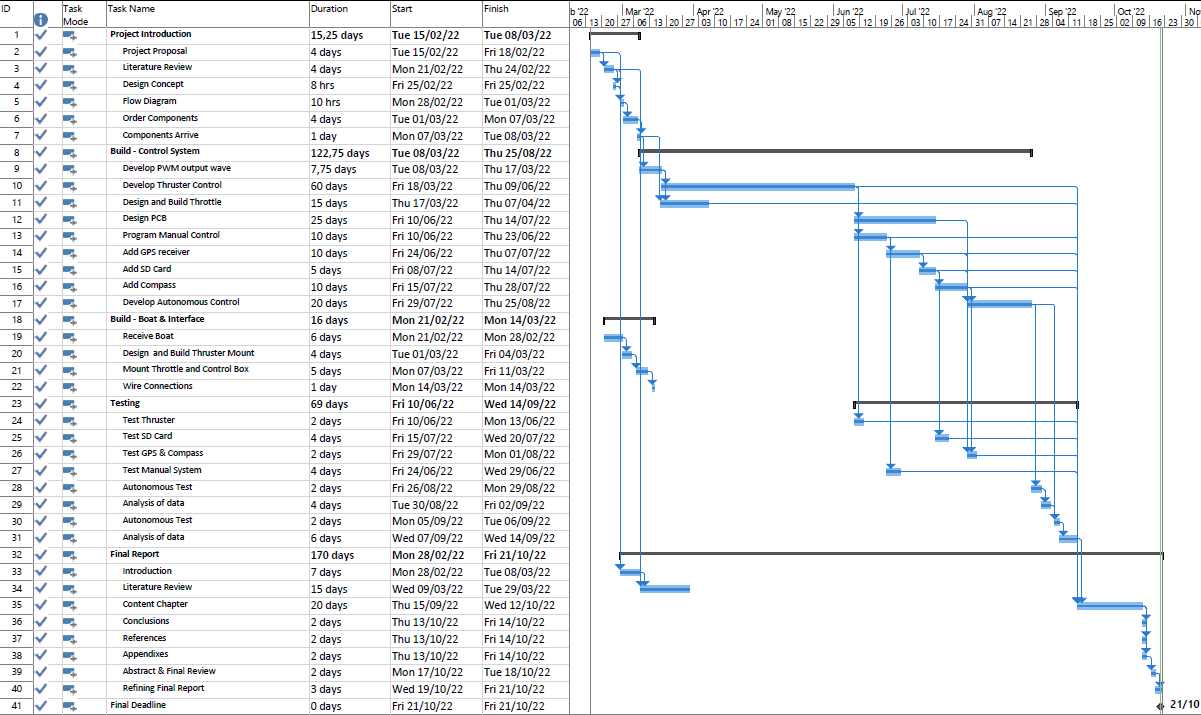
\includegraphics[width = \linewidth]{figures/Schedule.png}	


\end{landscape}
%\chapter{Safety Procedures}
The Stellenbosch Engineering laboratories were not used in this project however, once the prototype was developed there were several tests with the system on a dam. There are risks involved in this testing. Table \ref{saf} is the activity based risk assessment that shows the risks associated with the project and the mitigation taken to limit the effects of these risks. Overall the mitigations worked as there was risk occurrence. An incorrect connection was made leading to a short circuit and damaging the one ESC. 

\begin{table}
	\caption{Activity Based Risk Assessment}
	\label{saf}
\begin{tabular}{|m{2.5cm}|m{2.5cm}|m{1cm}|m{3cm}|m{6cm}|}
	\cl{1-5}
	\textbf{Activity} & \textbf{Risk} & \textbf{Risk Type} & \textbf{Classification of risk severety} &\textbf{ Mitigating Steps} \\
	\cl{1-5}
	\multirow{2}{2cm}{Launching Vessel} & Vessel sinking & E & Acceptable Risk & Ensure that the bungs are securely sealed \\
	\cl{2-5}
	& Vessel floating away & E & Acceptable Risk & Ensure a secondary rope is attached to the vessel to pull it back once it is off the trailer \\
	\cl{1-5}
	Connecting Electronic Equipment & Short Circuit & E & Substantial Risk & Double check which connection is the correct one before connecting them. \\
	\cl{1-5}
	Connecting Battery System & Electrical Shock & P & Possible Risk & Ensure the power switch is off before connecting the terminals and connect one terminal at a time and next touch both terminals. \\
	\cl{1-5}
	Operating Vessel & Cut limbs on thruster blades & P & Substantial Risk & Turn off the main power to the thruster before approaching the thrusters. \\
	\cl{2-5}
	& Electrical short & E & Substantial Risk & All connections are waterproofed to the best of abilities. \\
	\cl{2-5}
	& Vessel Collision & P\textbackslash{}E & Acceptable Risk & Be aware of surrounding and be ready to switch to manual control when operating the vessel. \\
	\cl{1-5}
	Moving around the vessel & Falling overboard & P & High Risk & Always wear a PFD while operating the vessel and keep a hold of the edges while moving around the vessel. \\
	\cl{2-5}
	& Capsizing vessel & P\textbackslash{}E & Possible Risk & Always wear a PFD while on the vessel and do not overload the vessel weight limit. \\
	\cl{1-5}
	Transporting vessel & Vehicle collision & P\textbackslash{}E & High Risk & Only a licensed driver may drive and must remain aware of the road conditions at all times. \\
	\cl{2-5}
	& Vessel trailer unhitching & P\textbackslash{}E & High Risk & Always ensure the vessel is securely hitched and check this routinely on long journeys. \\
	\cl{2-5}
	& Vessel falling off the trailer & P\textbackslash{}E & Substantial Risk & Always ensure the vessel is securely tied down when transporting. \\
	\cl{2-5}
	& Equipment falling off & E & Possible Risk & Secure the equipment in the vehicle and not on th vessel for transport. \\
	\cl{1-5}
\end{tabular}
\end{table}
%\chapter{Bill of Materials}
\label{BOM}

\backmatter%=========================================================

%\bibliography{USbibsample}
\bibliography{bib}

\end{document}
